%課題研究レジュメテンプレート ver. 1.2

\documentclass[uplatex]{jsarticle}
\usepackage[top=20mm,bottom=20mm,left=20mm,right=20mm]{geometry}
\usepackage[T1]{fontenc}
\usepackage{txfonts}
\usepackage{wrapfig}
\usepackage[expert,deluxe]{otf}
\usepackage[dvipdfmx,hiresbb]{graphicx}
\usepackage[dvipdfmx]{hyperref}
\usepackage{pxjahyper}
\usepackage{secdot}

\makeatletter
  \renewcommand{\section}{%
    \if@slide\clearpage\fi
    \@startsection{section}{1}{\z@}%
    {\Cvs \@plus.5\Cdp \@minus.2\Cdp}% 前アキ
    {.5\Cvs \@plus.3\Cdp}% 後アキ
    %{\normalfont\Large\headfont\raggedright}}
    {\normalfont\raggedright}}

  \renewcommand{\subsection}{\@startsection{subsection}{2}{\z@}%
    {\Cvs \@plus.5\Cdp \@minus.2\Cdp}% 前アキ
    {.5\Cvs \@plus.3\Cdp}% 後アキ
    %{\normalfont\large\headfont}}
    {\normalfont}}

  \renewcommand{\subsubsection}{\@startsection{subsubsection}{3}{\z@}%
    {\Cvs \@plus.5\Cdp \@minus.2\Cdp}%
    {\z@}%
    %{\normalfont\normalsize\headfont}}
    {\normalfont}}
\makeatother
%ここから上を編集する必要はない.





\title{\vspace{-14mm}プロジェクトで発生するリスクのMBTIを用いた事前予測}
\author{PMコース 矢吹研究室 1442085 中村真悟}
\date{}%日付を入れる必要はない.
\pagestyle{empty}%ページ番号は振らない.
\begin{document}
\maketitle


\section{研究の背景}

プロジェクトマネジメントとはヒト・モノ・カネ・資源を管理することである.この中で最もプロジェクトに関わり,かつ対処が確立しにくいのはヒトであると私は考える.

プロジェクトの定義においてメンバは固定されない.毎回初対面のメンバが必ずいるといっても過言ではない.ならば,プロジェクトマネージャがより早くメンバのことを,人間的特徴を把握することができればより良いマネジメントができるのではないか.

ユングの類型論を発展させたMBTI\cite{mbti}というものがある.人の考え方を
\begin{itemize}
\item 内向:I・外向:E
\item 感覚:S・直感:N
\item 思考:T・感情:F
\item 判断的態度:J・知覚的態度:P
\end{itemize}
の4指標の組み合わせで16タイプに分類するものである.この技法はキャリアカウンセリングやリーダーシップ開発,チームビルディングなどに使われることが多い\cite{mbti}.

このMBTIを用いて,プロジェクトのメンバの大まかな性格を理解し,メンバの相互作用が原因となって起きる事象を予測したい.
以上のことから本研究ではMBTIを用いて,プロジェクトを円滑に遂行する方法を研究する.




\section{研究の目的}

本研究の目的は,チームメンバのMBTIの16タイプの相互作用がプロジェクトにどのような影響をもたらしているのかを調べる.この結果から,MBTIのタイプに基づいてメンバ間で発生しやすいリスクを特定できるすることである.



\section{プロジェクトマネジメントの関連}

本研究は,PMBOKにおけるリスク・マネジメントに該当する.MBTIは自己理解メソッドであり自己成長を促すため,人的資源マネジメントにも関連している.また,MBTIはチームビルディングに用いることができる.さらにはメンバ間の円滑なコミュニケーション向上が期待できるため,MBTIはコミュニケーションマネジメントに応用できる.

\section{研究方法}

以下の手順で研究を進める.
\begin{itemize}
\item ソフトウェアコースのPM実験を受講する学生に対し,MBTIの性格検査を行いタイプを調査する
\item その学生に対し,アンケートを行い実際にどのような事象が起きたか調査する
\item アンケートの結果と個人のタイプでどのような関連があるのかを考察する
\end{itemize}


\section{現在の進捗状況}

上記の手順で,PM実験のソフトウェアコースを受講していた学生38人にMBTI診断とアンケート調査を行った.MBTI診断の結果は表\ref{wariai}の通りである.今回診断した学生38人で,16タイプ中13タイプがいた.

表\ref{ke1}\ref{ke2}は2×3集計表での相関関係を求めたものである.集計表は実際の生データを集計したものである.期待度の表は集計表の合計の結果をもとに算出された値である.この値は帰無仮説に基づいた2つの相関がない場合の値となる.値Zとは集計表と期待度のずれを計算したものである.この値Zの5%を下回るのであれば帰無仮説は棄却される.
この表において,pが値Zの5%を下回るため,相関があるということになる.

内向(I)型:外向(E)型と「情報共有は問題なくできていた」という質問の回答結果(表\ref{ke1})では値Zの5%の棄却域にあたる0.045を出したため,相関がある.この結果から「自分とは違うタイプがいると情報共有しにくい」傾向がある.
同じように規範(J)型:柔軟(P)型と「情報共有は問題なくできていた」という質問の回答結果(表\ref{ke2})では,「自分とは同じタイプがいると情報共有しにくい」傾向がある.


\begin{figure}[h]
   \begin{tabular}{c}

      % 1
      \begin{minipage}{0.33\hsize}
        \begin{center}
   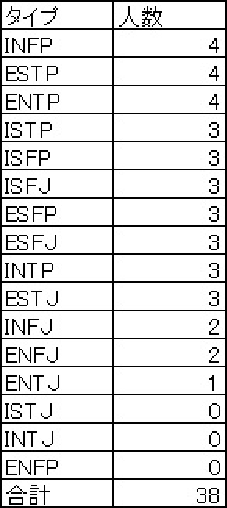
\includegraphics[width=3cm,clip]{wariai.pdf}
  \caption{MBTI結果}
  \label{wariai}
  \end{center}
 \end{minipage}

 \begin{minipage}{0.6\hsize}
   \begin{center}
  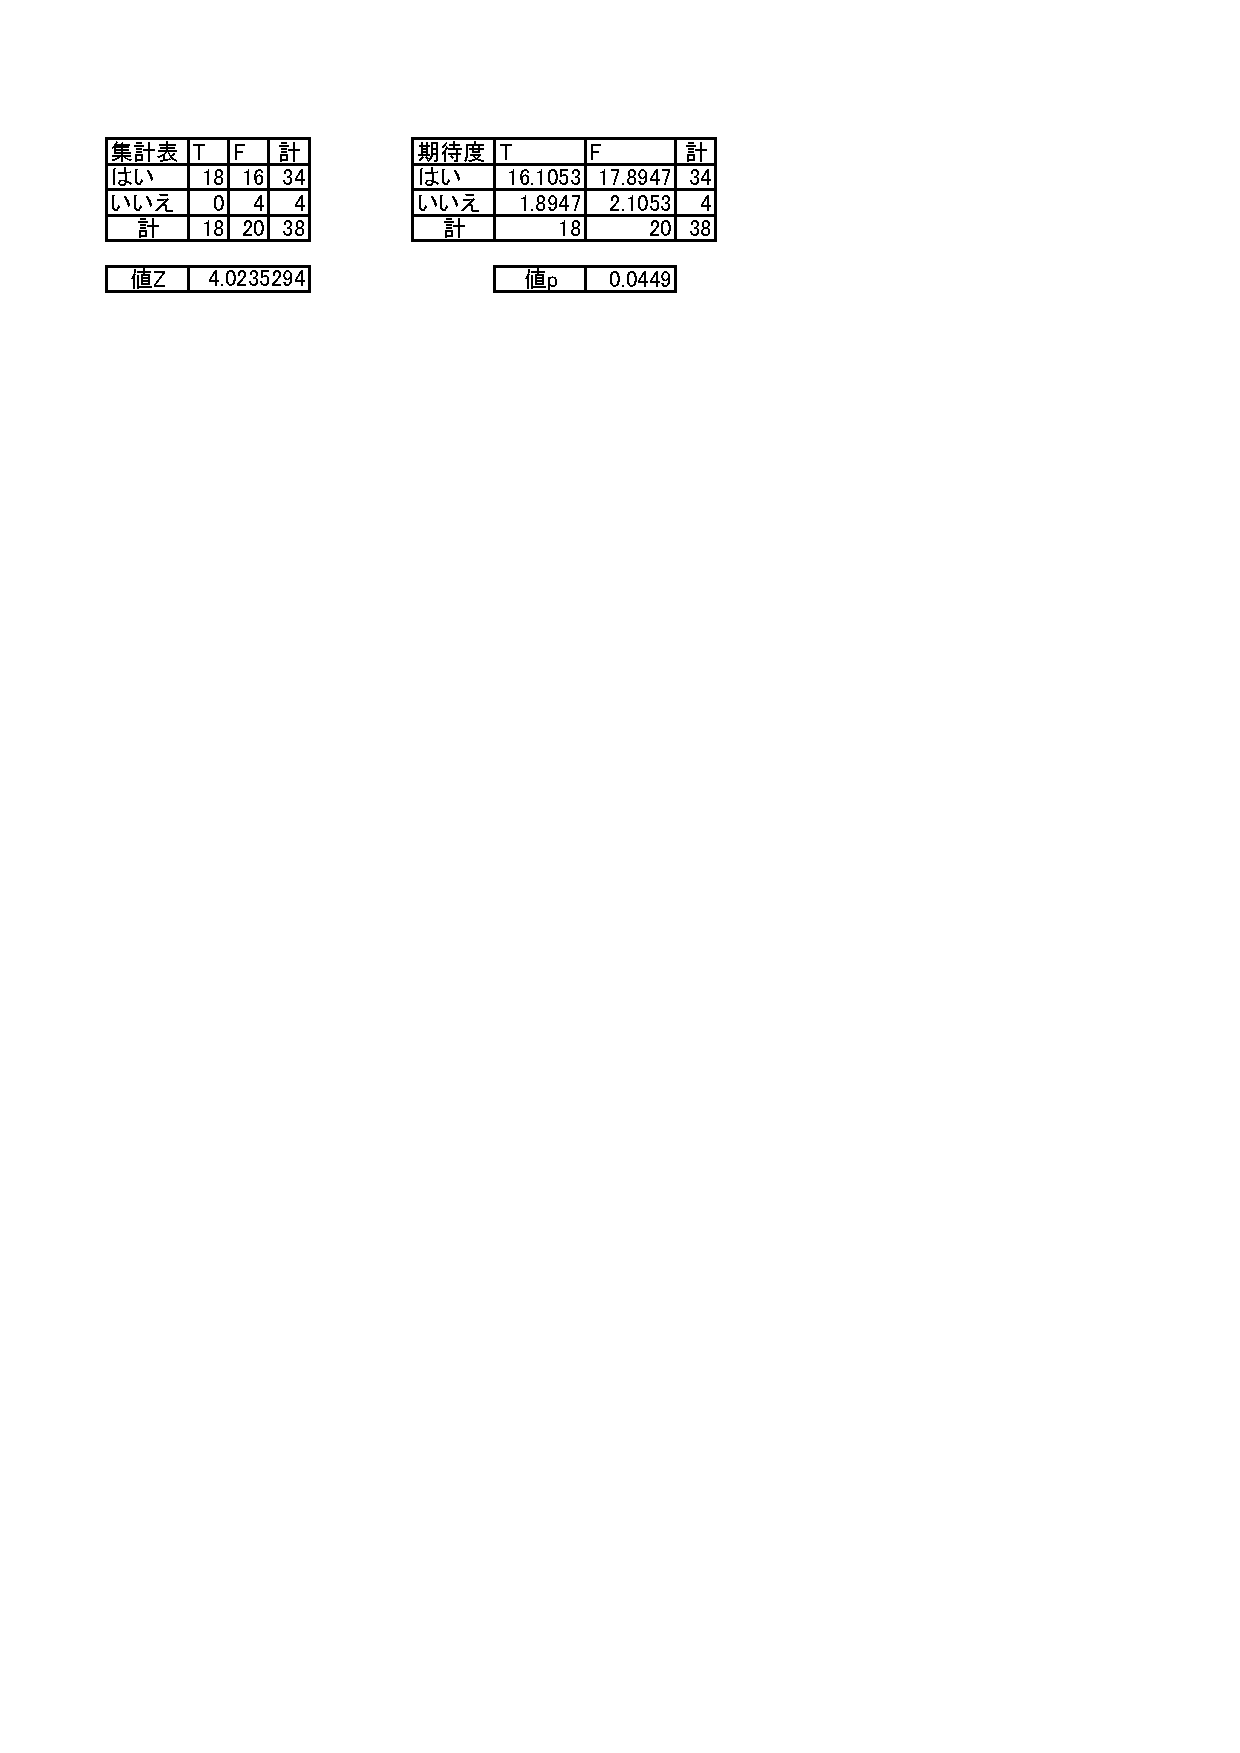
\includegraphics[width=8.2cm,clip]{kekka.pdf}
  \caption{I・Eの関係と情報共有したかの回答結果のクロス集計}
  \label{ke1}
   \end{center}
    \begin{center}  
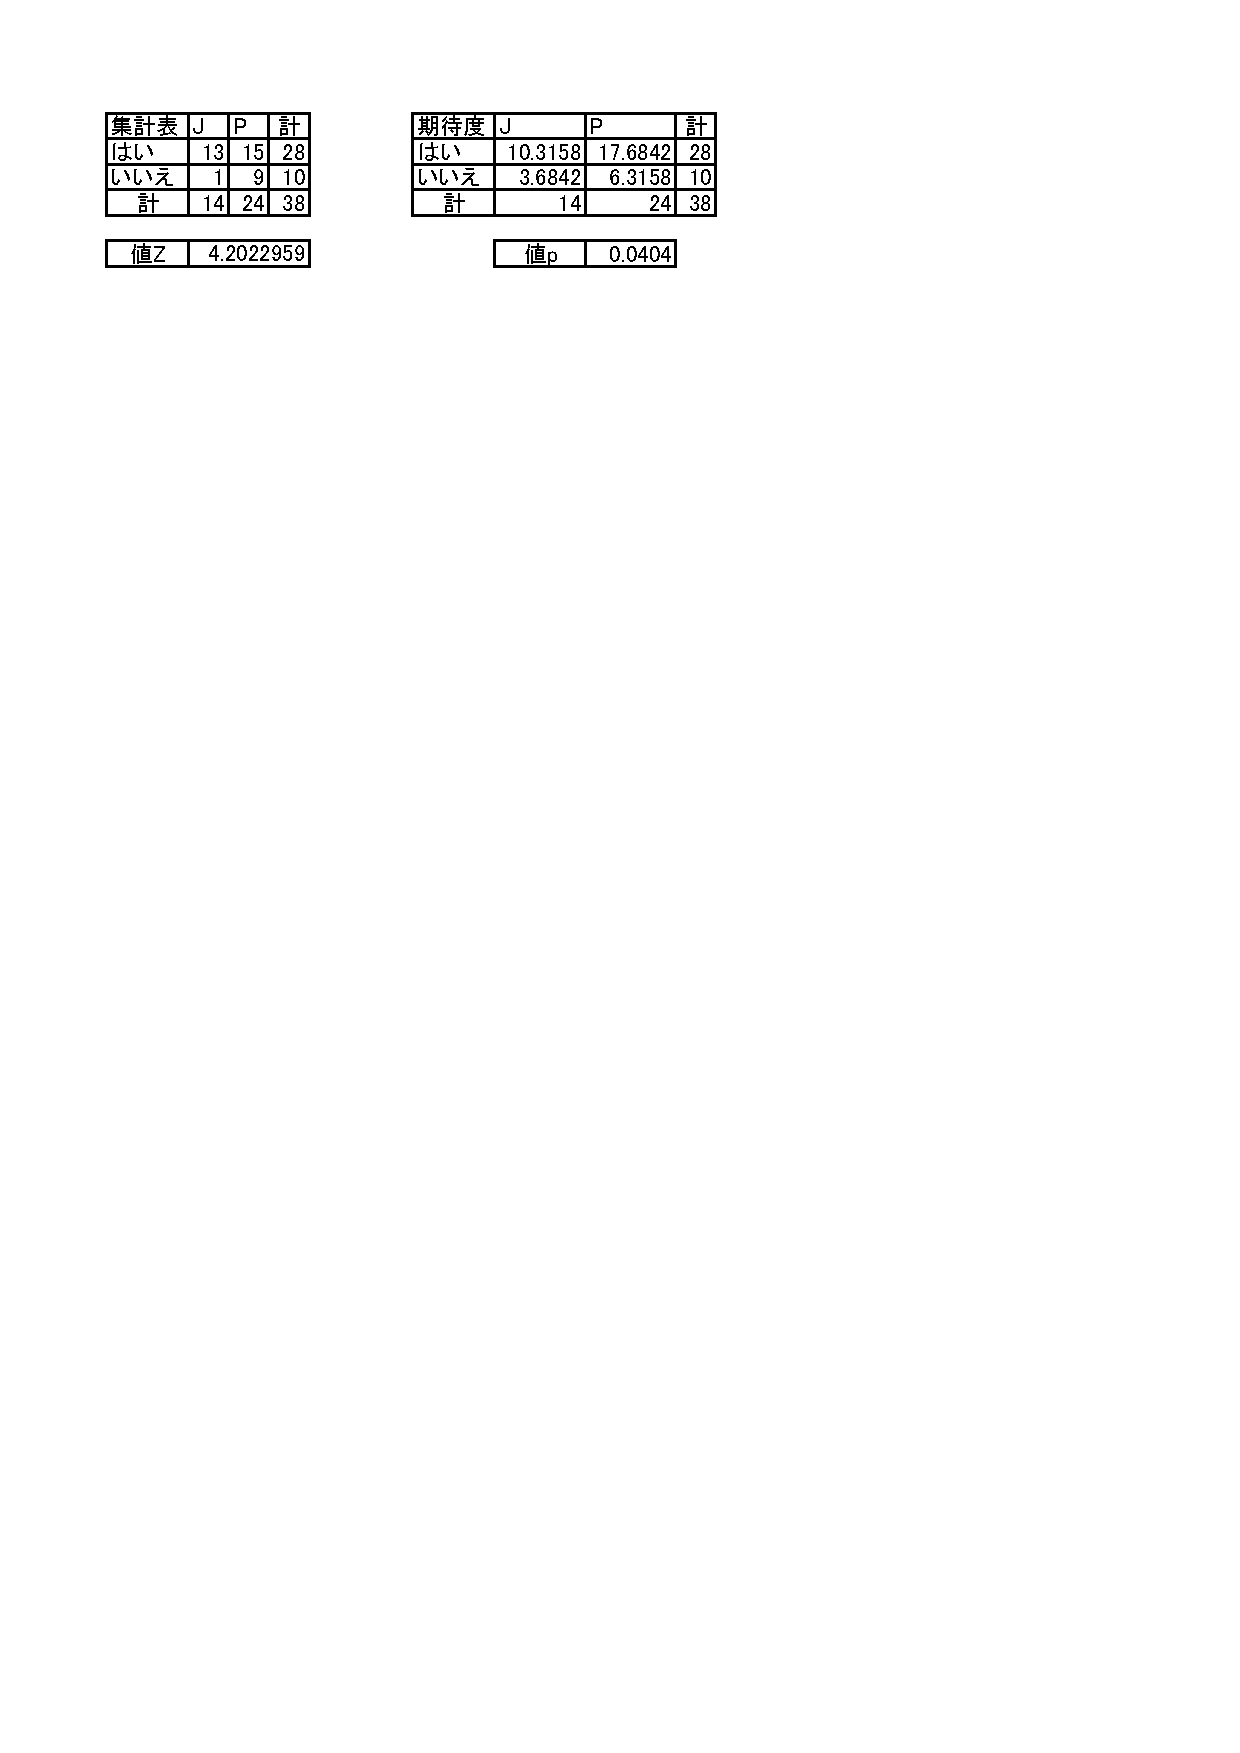
\includegraphics[width=8.2cm,clip]{kekka2.pdf}
  \caption{J・Pの関係と情報共有したかの回答結果のクロス集計}
  \label{ke2}
   \end{center}
 \end{minipage}
\end{tabular}
  \end{figure}


\section{今後の計画}
以下の手順で計画を進める.
\begin{itemize}
\item 今回のアンケート結果を踏まえ,アンケートの項目を増やす
\item PM演習を受講する学生に対し同様の方法でアンケートを行い検証する.
\item PM演習の間3回,発表後1回アンケートを行う.
\end{itemize}




\nocite{BB19543658}\nocite{110003745117}\nocite{ylab2015}\nocite{katolab2015}
\bibliographystyle{junsrt}
\bibliography{biblio}%「biblio.bib」というファイルが必要.

\end{document}